\hypertarget{technical-fork}{%
\subsubsection{Technical Fork}\label{technical-fork}}

Question: What are a number of technical forks of an open source project
on code development platforms?

\hypertarget{description}{%
\paragraph{Description}\label{description}}

A technical fork is a distributed version control copy of a project. The
number of technical forks indicates the number of copies of a project on
the same code development platform.

\hypertarget{objectives}{%
\paragraph{Objectives}\label{objectives}}

The objective of the Technical Fork metric is to ascertain how many
copies of a project exist on a code development platform. Analysis of
technical forks may provide insight into forking intentions (different
types of forks such as contributing, and non-contributing forks).

\hypertarget{implementation}{%
\paragraph{Implementation}\label{implementation}}

\hypertarget{filters}{%
\subparagraph{Filters}\label{filters}}

\begin{itemize}
\tightlist
\item
  Time Period (e.g., Weekly, Monthly, Annually)
\item
  Ratio of contributing fork to total forks (A contributing fork is a
  fork that has opened a change request against the original
  repository.)
\item
  Ratio of non-contributing fork to total forks (A non-contributing fork
  is a fork that has never opened a change request against the original
  repository.)
\end{itemize}

\hypertarget{visualizations}{%
\subparagraph{Visualizations}\label{visualizations}}

\textbf{Augur Implementation}\\
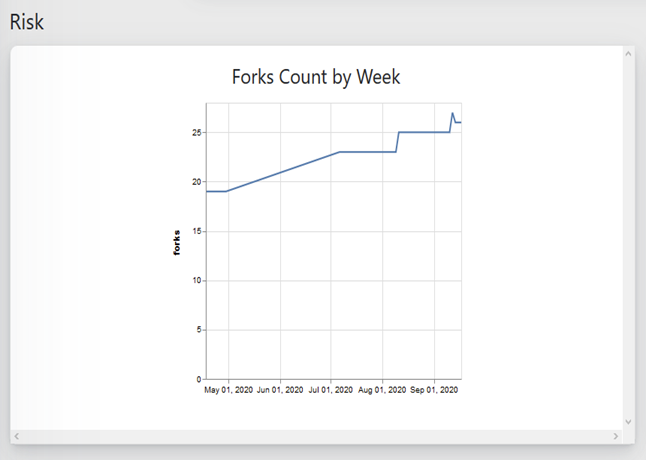
\includegraphics{images/technical-fork_augur-fork.png}

\textbf{GrimoireLab Implementation}\\
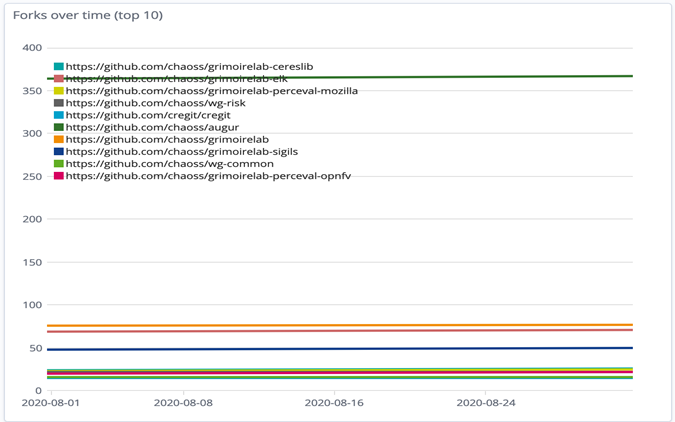
\includegraphics{images/technical-fork_grimoirelab-fork.png}

\hypertarget{tools-providing-the-metric}{%
\subparagraph{Tools Providing the
Metric}\label{tools-providing-the-metric}}

\begin{itemize}
\tightlist
\item
  Augur
\item
  GrimoireLab
\end{itemize}

\hypertarget{data-collection-strategies}{%
\subparagraph{Data Collection
Strategies}\label{data-collection-strategies}}

\textbf{Github API}\\
\url{https://developer.github.com/v3/repos/forks/\#list-forks}

\textbf{GitLab API}\\
\url{https://docs.gitlab.com/ee/api/projects.html\#list-forks-of-a-project}

\textbf{Bitbucket API}\\
\url{https://developer.atlassian.com/bitbucket/api/2/reference/resource/repositories/\%7Bworkspace\%7D/\%7Brepo_slug\%7D/forks}

\hypertarget{references}{%
\paragraph{References}\label{references}}

\url{https://help.github.com/en/enterprise/2.13/user/articles/fork-a-repo}
\url{https://opensource.com/article/17/12/fork-clone-difference}
